% mnras_template.tex 
%
% LaTeX template for creating an MNRAS paper
%
% v3.0 released 14 May 2015
% (version numbers match those of mnras.cls)
%
% Copyright (C) Royal Astronomical Society 2015
% Authors:
% Keith T. Smith (Royal Astronomical Society)

% Change log
%
% v3.0 May 2015
%    Renamed to match the new package name
%    Version number matches mnras.cls
%    A few minor tweaks to wording
% v1.0 September 2013
%    Beta testing only - never publicly released
%    First version: a simple (ish) template for creating an MNRAS paper

%%%%%%%%%%%%%%%%%%%%%%%%%%%%%%%%%%%%%%%%%%%%%%%%%%
% Basic setup. Most papers should leave these options alone.
\documentclass[fleqn,usenatbib]{mnras}

% MNRAS is set in Times font. If you don't have this installed (most LaTeX
% installations will be fine) or prefer the old Computer Modern fonts, comment
% out the following line
\usepackage{newtxtext,newtxmath}
% Depending on your LaTeX fonts installation, you might get better results with one of these:
%\usepackage{mathptmx}
%\usepackage{txfonts}

% Use vector fonts, so it zooms properly in on-screen viewing software
% Don't change these lines unless you know what you are doing
\usepackage[T1]{fontenc}

% Allow "Thomas van Noord" and "Simon de Laguarde" and alike to be sorted by "N" and "L" etc. in the bibliography.
% Write the name in the bibliography as "\VAN{Noord}{Van}{van} Noord, Thomas"
\DeclareRobustCommand{\VAN}[3]{#2}
\let\VANthebibliography\thebibliography
\def\thebibliography{\DeclareRobustCommand{\VAN}[3]{##3}\VANthebibliography}


%%%%% AUTHORS - PLACE YOUR OWN PACKAGES HERE %%%%%

% Only include extra packages if you really need them. Common packages are:
\usepackage{graphicx}	% Including figure files
\usepackage{amsmath}	% Advanced maths commands
\usepackage{amssymb}	% Extra maths symbols

%%%%%%%%%%%%%%%%%%%%%%%%%%%%%%%%%%%%%%%%%%%%%%%%%%

%%%%% AUTHORS - PLACE YOUR OWN COMMANDS HERE %%%%%
\DeclareMathOperator*{\argmin}{arg\,min}
\DeclareMathOperator*{\argmax}{arg\,max}
% Please keep new commands to a minimum, and use \newcommand not \def to avoid
% overwriting existing commands. Example:
%\newcommand{\pcm}{\,cm$^{-2}$}	% per cm-squared

%%%%%%%%%%%%%%%%%%%%%%%%%%%%%%%%%%%%%%%%%%%%%%%%%%

%%%%%%%%%%%%%%%%%%% TITLE PAGE %%%%%%%%%%%%%%%%%%%

% Title of the paper, and the short title which is used in the headers.
% Keep the title short and informative.
\title[Importance sampling with normalizing flows]{Rapidly combining cosmological probes with importance sampling and normalizing flows }

% The list of authors, and the short list which is used in the headers.
% If you need two or more lines of authors, add an extra line using \newauthor
\author[B. Thorne]{
B. Thorne,$^{1}$\thanks{E-mail: blthorne@ucdavis.edu}
L. Knox,$^{1}$
\\
% List of institutions
$^{1}$Department of Physics, University of California, One Shields Avenue, Davis, CA 95616, USA\\
}

% These dates will be filled out by the publisher
\date{Accepted XXX. Received YYY; in original form ZZZ}

% Enter the current year, for the copyright statements etc.
\pubyear{2021}

% Don't change these lines
\begin{document}
\label{firstpage}
\pagerange{\pageref{firstpage}--\pageref{lastpage}}
\maketitle

% Abstract of the paper
\begin{abstract}
This is an abstract
\end{abstract}

% Select between one and six entries from the list of approved keywords.
% Don't make up new ones.
\begin{keywords}
keyword1 -- keyword2 -- keyword3
\end{keywords}

%%%%%%%%%%%%%%%%%%%%%%%%%%%%%%%%%%%%%%%%%%%%%%%%%%

%%%%%%%%%%%%%%%%% BODY OF PAPER %%%%%%%%%%%%%%%%%%

\section{Introduction}

\begin{itemize}
    \item Difficulty of importance sampling in datasets with poor coverage of true posterior
    \item General applicability to Bayesian inference: MCMC techniques etc
\end{itemize}

\section{Methods}

\subsection{Normalizing Flows}
\label{sec:normalizing_flows} % used for referring to this section from elsewhere

Normalizing flows have gained much attention in recent years for their ability to model complicated posterior distributions in terms of simple, tractable base distributions. Typically, they have been applied in the machine learning community to model the distributions of datasets such as natural images \citep{ho/etal:2019, grathwohl/etal:2018, kingma/dhariwal:2018}, video \citep{kumar/etal:2019}, and audio \citep{kim/etal:2018}. 

{\textbf More intro here}

For a continuous random variable, $x\in \mathbb R^d$ we construct a flexible family of functions $q_\phi(x)$, parametrized by $\phi$. Normalizing flows provide a framework for defining the family $q_\phi(x)$, and inferring the parameters $\phi$. and  normalizing flows, for additional details we refer readers to reviews of this subject \citep{kobyzev/etal:2019, papamakarios/etal:2019}.

The central idea is to start with a simple base distribution over a random variable $z\in\mathbb R^d$ from which we can easily draw samples $z \sim p_z(z)$. In practice this is often a multivariate Gaussian. A normalizing flow then transforms this density to the density of interest $p(x)$:
\begin{equation}
    z = f(x), \quad {\rm with} \quad x \sim p(x). 
\end{equation}
In order for this transformation to be a \emph{flow}, we require $f$ to be invertible, and for both its forward and reverse directions to be differentiable. One can think of this transformation as stretching and shaping the simple space in order to fit a more complicated distribution. The details of this distortion are encoded by the Jacobian of the transformation:
\begin{equation}
J_f(x) = \begin{pmatrix}
    \frac{\partial f_1}{\partial x_1} & \dots & \frac{\partial T_1}{\partial x_d} \\
    \vdots & \ddots & \vdots \\
    \frac{\partial f_d}{\partial x_1} & \dots & \frac{\partial f_d}{\partial x_d} \\
\end{pmatrix}.
\end{equation}
The log likelihood of $x$ can then be written in terms of the base density and the Jacobian of the transformation by a change of variables:
\begin{equation}
\label{eq:log_prob}
    \log p(x) = \log p_z(f(x)) + \log | \det J_f(x) |.
\end{equation}
In principle, if the transformation $f$ is sufficiently flexible, we could approximate any distribution $p(x)$ in this way. Typically, $f$ is taken to be a neural network $f_\phi$, with some weights $\phi$. In order to make this transformation as flexible as possible, layers of simple networks are composed, taking advantage of the fact that compositions of invertible, differentiable functions are themselves invertible and differentiable. We can denote the overall transformation as:
\begin{equation}
z = f^n_{\phi_n} \circ f^{n-1}_{\phi_{n-1}} \circ \dots \circ f^1_{\phi_1}(x) \equiv f_\phi(x),
\end{equation}
where $f^i_{\phi_i}$ is the $i^{\rm th}$ transformation. Using this parametrization, the transformed density is:
\begin{equation}
    \log q_\phi(x) = \log p_z(f_\phi(x)) + \sum_{i=1}^n \log \det J_{f^i}(x).
\end{equation}
In order for the transformed density to be computationally efficient we require the calculation of $f_\phi(x)$ to be parallelizable, and for the Jacobian determinants to be computationally efficient. These are key constraints on the permissible network designs when constructing normalizing flows \cite{rezende/etal:2015, papamakarios/etal:2019}. A typical choice is to use so-called \emph{autoregressive} networks, which have the nice property of satisfying both of these constraints.

TODO:
\begin{itemize}
\item[i)] Describe planar and radial flows, NICE architectures, MADE, MAF, and IAF
\item[ii)] Explain parametrization we chose and maximization objective.
\end{itemize}


With the network structure determined, we now turn to the process of determining the weights $\phi$. Taking the target distribution $p(x)$, we would like to optimize our approximation $q_\phi(x)$ by adjusting the parameters $\phi$. To do this, we minimize the Kullback-Leibler (KL) divergence between the two distributions:
\begin{equation}
\label{eq:kl_divergence}
    \mathbb{D}_{\rm KL}(p(x) || q_\phi(x)) = \int p(x) \log\left(\frac{p(x)}{q_\phi(x)}\right)dx.
\end{equation}
The KL divergence is a measure of the `distance' between two distributions, and is positive when the distributions are not exactly equal, or zero when they are exactly equal. The optimal network weights, $\hat \phi$, minimize the KL divergence:
\begin{equation}
    \hat \phi = \argmin_\phi~\mathbb D_{\rm KL}(p(x) || q_\phi(x)).
\end{equation}
Expanding the log term in Equation~\ref{eq:kl_divergence}, and discarding the term that does not depend on the weights $\phi$, we can write this as:
\begin{equation}
\label{eq:max_lkl}
\begin{aligned}
    \hat \phi &= \argmax_\phi~\int p(x) \log q_\phi(x) dx \\
              &= \argmax_\phi~\mathbb E_{x\sim p(x)}[\log q_\phi(x)].
\end{aligned}
\end{equation}
In this form we can see that minimizing the KL divergence is equivalent to maximizing the log likelihood of the model over samples from the true underlying distribution. In the application we are pursuing, we have access to well-converged MCMC chains containing many samples from the true posterior, and we can make Monte Carlo estimates of the expectation in Equation~\ref{eq:max_lkl}. Our algorithm for learning the weights $\phi$ will therefore be as follows:
\begin{itemize}
    \item[i)] Initialize a normalizing flow $q_\phi(x)$ with architecture described in Section~\ref{sec:normalizing_flows}.
    \item[ii)] For mini-batches of the data, compute Monte Carlo estimates of the expectation in Equation~\ref{eq:max_lkl}.
    \item[iii)] Compute gradients of the expectation with respect to network weights, and update $\phi$.
    \item[iv)] Repeat (iii) until $\phi$ converges, this final value is $\hat \phi$.
\end{itemize}

In Section~\ref{sec:importance_sampling} we describe how the rapid generation of samples from the trained flow allows for the fast combination of trained posteriors with additional datasets via \emph{importance sampling}, and we present the results of this application in Section~\ref{sec:results}. However, the flexibility of this approach admits many new possibilities such as efficient, scalable MCMC sampling with Hamiltonian Monte Carlo \citep{hoffman/etal:2019}, improving the generative modeling of astronomical images \citep{thorne/etal:2021, kingma/etal:2016}   We discuss the potential application of these methods further in Section~\ref{sec:conclusions}.

\subsection{Importance Sampling}
\label{sec:importance_sampling}

\emph{Importance sampling} (IS) is often used in the analysis of cosmological data sets as it allows for quick comparison of parameter constraints when conditioning on additional data, or checking the influence of priors, without needing to run additional, computationally expensive, MCMC chains \citep{lewis/bridle:2002}. IS allows one to compute expectation values with respect to a new distribution by re-weighing samples from a previously-run MCMC chain, using a weight factor proportional to the new posterior value at each sampled point. The main drawback to this approach is that the new posterior can not be far away from the existing posterior, or be overly constraining. In either of these cases importance-sampled constraints may suffer from high variance due to a limited number of samples with significant weight. In this paper we propose using a trained normalizing flow, from which we may generate many samples very quickly, to improve the accuracy of constraints derived by importance sampling. In the rest of this section we will describe the specifics of importance sampling. 

If the posterior approximation is not normalized, such that $\int q(x)dx = Z$, then we can account for this in the reweighting procedure:

\begin{itemize}
\item[i)] we can sample $x$ by first sampling $z \sim p(z)$ and pushing this through the transformation: $x = f(z)$, 
\item[ii)] Evaluating the log probability for a given $x$, which requires calculating the inverse transformation $z = f^{-1}(x)$ as well as the log determinant of the Jacobian in Equation \ref{eq:log_prob}, and the log probability of the base distribution $q(z)$.  
\end{itemize}

\subsection{Importance Transfer}
\label{sec:importance_transfer}

In this section we will propose a technique to use importance sampling to approximate an unknown distribution as another normalizing flow. Consider a distribution $p(x)$ which we are not able to sample from, but which we are able to evaluate. Such a situation arises frequently in importance sampling. We may consider an approximation to this distribution using a normalizing flow, as in Section~\ref{sec:normalizing_flows}, however we would not be able to train this flow in the same way, as we have no access to samples. To make progress, let us revisit the objective function in Equation~\ref{eq:max_lkl}. Note that we can not directly evaluate the expectation value in Equation~\ref{eq:max_lkl}, but using importance sampling we may approximate it:
\begin{equation}
\begin{aligned}
\mathbb E_{x\sim p(x)}[\log q_\phi(x)] &= \int p(x) \log q_\phi(x) dx \\
    &= \int q_\phi(x) \frac{p(x)}{q_\phi(x)} \log q_\phi(x) dx
\end{aligned}
\end{equation}


\section{Data}
\label{sec:data}

In this section we will describe the data products used to train the normalizing flow outlined in Section~\ref{sec:normalizing_flows}, and the data products that will be used in the importance sampling process.

\subsection{CMB Data}

To train the normalizing flow, we use publicly available MCMC chains from the Planck 2018 analysis. For the training process we take the {\tt Plik\_TTTEEE\_lowl+lowE} posterior samples, and to validate our approac we compare the importance-sampled values to those derived from the {\tt Plik\_TTTEEE\_lowl+lowE+BAO} likelihood.

\subsection{BAO Data}
\label{sec:bao_data}

Baryon acoustic oscillations (BAOs) provide a \emph{standard ruler} that may be used to measure the expansion history of the Universe. At recombination, acoustic waves travelling through the photon-baryon plasma are frozen into the matter distribution, defining a characteristic scale that is present both in the CMB, and in the low-redshift distribution of galaxies.

\begin{equation}
    r_{\rm drag} = \int_{z_*}^\infty \frac{c_s(z)}{H(z)} dz
\end{equation}

This characteristic scale shows up as a sharp feature in the correlation function of galaxies at the comoving sound horizon scale, $r_s$, or as an oscillatory feature in their power spectrum, well above the virialization scale at which non-linear physics becomes important. The measurement of the BAO scale therefore provides a robust model-independent measurement of the expansion rate and angular diameter distance as a function of redshift. 
\begin{equation}
\begin{aligned}
    &\frac{D_A(z)}{r_{\rm drag}} = \frac{c}{r_{\rm drag}}\int_0^z \frac{dz}{H(z)} \\
    &H(z)\frac{r_{\rm drag}}{c} = \frac{r_{\rm drag}}{c}H(z)
\end{aligned}
\end{equation}
We will use the BAO contraints of \cite{alam/etal:2017}, expressed as Gaussian constraints on the quantities in Equation~ at three effective redshifts.




\section{Results}

\begin{figure*}
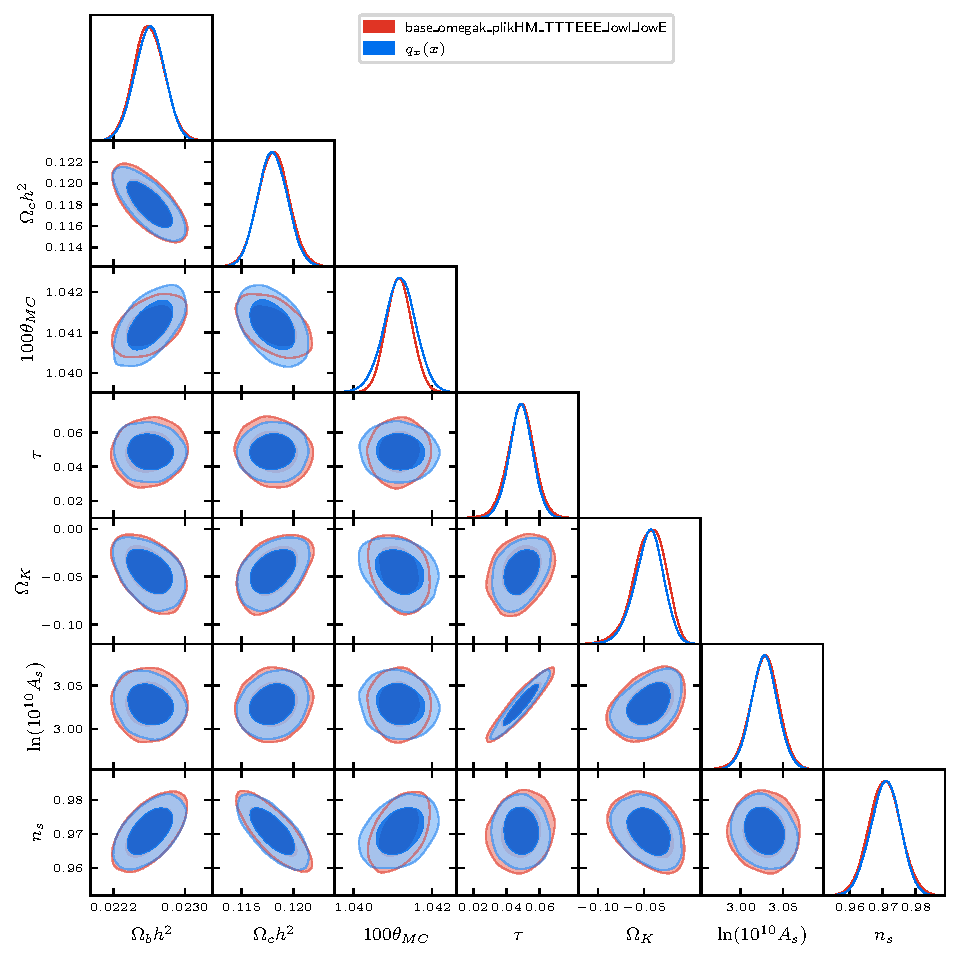
\includegraphics[]{./results/densities/corner.pdf}
\end{figure*}

\label{sec:results}


\section{Conclusions \& Discussion}
\label{sec:conclusions}


\section*{Acknowledgements}

We acknowledge the use of the GPU allocation at NERSC.

%%%%%%%%%%%%%%%%%%%%%%%%%%%%%%%%%%%%%%%%%%%%%%%%%%
\section*{Data Availability}

 
All the data used in this study is available on the Planck Legacy Archive: \url{https://pla.esac.esa.int/#home}.




%%%%%%%%%%%%%%%%%%%% REFERENCES %%%%%%%%%%%%%%%%%%

% The best way to enter references is to use BibTeX:

\bibliographystyle{mnras}
\bibliography{library} % if your bibtex file is called example.bib


% Alternatively you could enter them by hand, like this:
% This method is tedious and prone to error if you have lots of references
%\begin{thebibliography}{99}
%\bibitem[\protect\citeauthoryear{Author}{2012}]{Author2012}
%Author A.~N., 2013, Journal of Improbable Astronomy, 1, 1
%\bibitem[\protect\citeauthoryear{Others}{2013}]{Others2013}
%Others S., 2012, Journal of Interesting Stuff, 17, 198
%\end{thebibliography}

%%%%%%%%%%%%%%%%%%%%%%%%%%%%%%%%%%%%%%%%%%%%%%%%%%

%%%%%%%%%%%%%%%%% APPENDICES %%%%%%%%%%%%%%%%%%%%%

\appendix

\section{Some extra material}

If you want to present additional material which would interrupt the flow of the main paper,
it can be placed in an Appendix which appears after the list of references.

%%%%%%%%%%%%%%%%%%%%%%%%%%%%%%%%%%%%%%%%%%%%%%%%%%


% Don't change these lines
\bsp	% typesetting comment
\label{lastpage}
\end{document}

% End of mnras_template.tex
